\chapter{Programa}\label{cap:programa}

\section{Introdução}

Este capítulo descreve o programa desenvolvido para implementar o algoritmo de
controle proposto no capítulo~\ref{cap:modelagem}, bem como as APIs e programas
utilizados adicionalmente para possibilitar a execução de testes comparativos.

Na seção~\ref{sec:arq_prog} uma arquitetura simplificada do sistema de controle é apresentada.
Por sistema de controle, entenda-se o processo que vai desde a aquisição dos
dados da visão, planejamento e trasmissão dos comandos aos robôs.

Na seção~\ref{sec:minimax} uma implementação do algoritmo de controle conceitualizado no
capítulo~\ref{cap:modelagem} é apresentada.

Na seção~\ref{sec:pyroboime} o programa pyroboime é descrito.

Na seção~\ref{sec:metricas} são propostas métricas para comparar o algoritmo
proposto com o utilizado anteriormente.

\section{Arquitetura do programa}\label{sec:arq_prog}

Um modelo simplificado da arquitetura do sistema de controle utilizado no para
o desenvolvimento deste projeto é apresentado na figura~\ref{fig:arq_prog}.

\begin{figure}
  \centering
  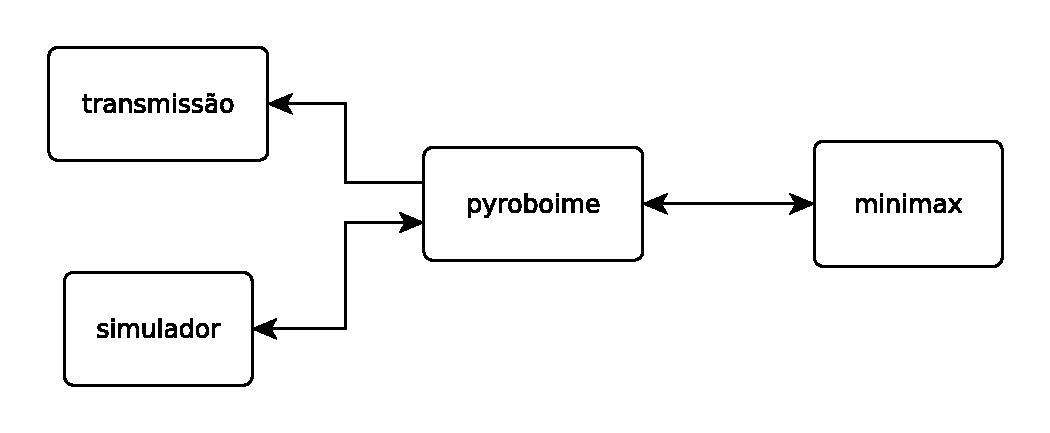
\includegraphics[width=0.8 \linewidth]{img/arq_geral_prog}
  \caption{Arquitetura simplificada do sistema de controle}\label{fig:arq_prog}
\end{figure}

\section{Processo do Minimax}\label{sec:minimax}
% disclaim: I don't think this is a good name ether...

O fluxo do programa é apresentado na figura~\ref{fig:minimax_flow}.

\begin{figure}
  \centering
  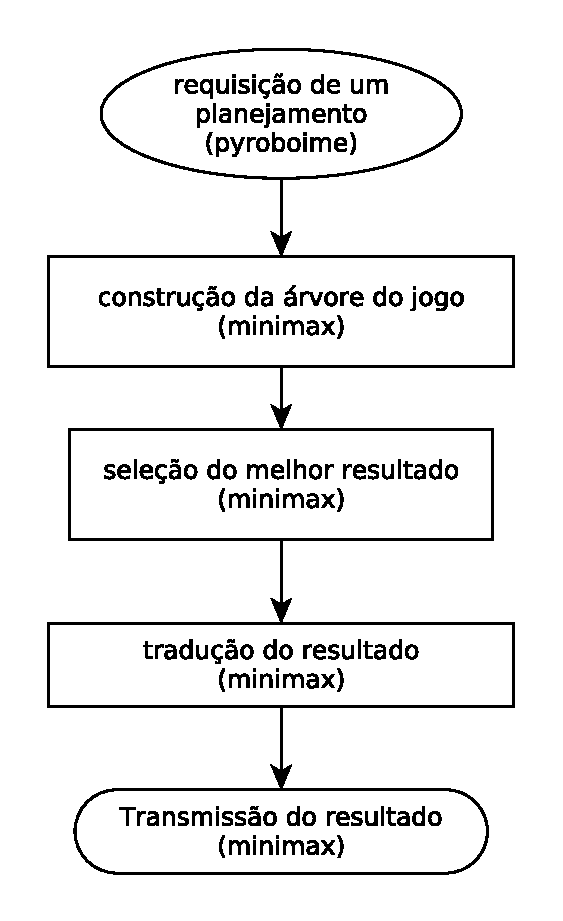
\includegraphics[width=0.2 \linewidth]{img/minimax_flow}
  \caption{Fluxo do processo minimax}\label{fig:minimax_flow}
\end{figure}

O processo de tradução consiste em transformar o planejamento obtido em uma
mensagem a ser enviada para o programa pyroboime. Para isso, foi utilizado
o protobuf. A estrutura do protocolo de resposta é apresentada no
arquivo~\ref{alg:minimax_resp_proto}. A estrutura do protocolo de atualização do
estado do tabuleiro apresentada no arquivo~\ref{alg:minimax_req_proto}.

Para otimizar os cálculos foi utilizada a API armadillo.

% Arquivo de resposta
\lstinputlisting [caption={Arquivo de definição do protocolo de resposta},
label={alg:minimax_resp_proto}] {prototypes/minimax/proto/discrete.proto}

% Arquivo de requisição
\lstinputlisting [caption={Arquivo de definição do protocolo de atualização do
  estado do tabuleiro},
label={alg:minimax_req_proto}] {prototypes/minimax/proto/update.proto}

\section{Pyroboime}\label{sec:pyroboime}
% disclaim: google translate of tdp software file

O projeto pyroboime atualmente é responsável pela inteligência artificial do
sistema de controle. Ele é baseado na arquitetura STP (\textit{Skill-Tactic-Play}
implementada em python.
Ele é composto pelo seguintes componentes: interface com a ssl-vision,
ssl-refbox e grSim, também possui um módulo de comunicação interno para o
sistema de transmissão via rádio.

O STP é uma arquitetura de três camadas, onde o nível mais baixo, habilidades,
permite as manipulações de baixo nível em um único robô. A camada do meio,
tácticas, faz uso da camada de habilidade de executar nível mais elevado
comportamento, possivelmente permitindo coopration, mas ainda atuando em um
único robô. A camada superior, jogos, coordena as táticas associadas a cada
robô. Para maximizar o desempenho, cada jogo é implementado para se comportar de
acordo com estados específicos: parada, parada, chutes indiretos e reprodução normal. 
Uma camada de nível superior implmented como um jogo alterna entre outras peças
baseadas em o estado atual árbitro.
%Esta arquitetura é melhor representado na figura ~ \ ref {fig: stp}.
                                                                                
Há também uma habilidade implementado entradas para redireccionar a partir de um
joystick tal que é possível testar o robô com pouco esforço.
                                                                                
A interface é estruturado como uma pilha de filtro que liga o AI para uma
cobrança flexível de atualizadores (que recebe informações de estado) e
  comandantes (que entregam comandos aos robôs, em ambos os ambientes simulados
e reais).
Ele abstrai o ambiente externo, onde o jogo é jogado a partir do AI \ @.
Entre os filtros na referida pilha é um filtro de Kalman que reduz o ruído vindo
a partir dos dados atualizador.
                                                                                                                                                                                                                                         
As interfaces do sistema de rádio trasmitter embutidos com libusb para controlar
o hardware do transmissor, o qual está ligado por USB.
\section{Métricas de avaliação}\label{sec:metricas}
% vim: tw=80 et ts=2 sw=2 sts=2
